\section{Propósito y alcance de la auditoría}
La preparación de un modelo de abandono requiere establecer qué representan las
filas, cómo se relacionan las fuentes y cuáles observaciones permiten reconstruir
una trayectoria temporal. En este sentido, el estudio auditó las siete tablas CSV
disponibles en la carpeta de datos, como parte del objetivo específico 1 y de la fase
de comprensión de los datos de CRISP-DM. La revisión corresponde al notebook
\texttt{01\_carga\_exploracion.ipynb}; sus resultados se obtuvieron mediante una
ejecución nueva y no mediante la reutilización de salidas históricas.

El descriptor de OULAD identifica información de matrícula, evaluaciones e
interacciones agregadas con recursos virtuales \cite{sdata2017171}. El presente
informe examina su consistencia en los archivos locales. La comprobación de huellas
SHA-256 permite reconocer los archivos utilizados y verificar que se conservaron
intactos durante el procesamiento; no sustituye una certificación de procedencia.

\section{Estructura y unidad de análisis}
Se verificaron 32\,593 inscripciones correspondientes a 28\,785 personas, 7 módulos y 22 combinaciones de módulo y presentación. La inscripción se identifica mediante la clave compuesta de estudiante, módulo y presentación. Se encontraron 3\,538 personas con más de una inscripción; por ello, el tamaño de la tabla no debe presentarse como número de estudiantes distintos.

\Needspace{0.23\textheight}\begingroup\small\setlength{\tabcolsep}{3pt}\renewcommand{\arraystretch}{1.16}
\begin{longtable}{>{\raggedright\arraybackslash}p{0.56\linewidth}>{\raggedright\arraybackslash}p{0.23\linewidth}>{\raggedright\arraybackslash}p{0.15\linewidth}}
\caption{Dimensiones verificadas de las fuentes locales.}\label{rev01:dimensiones}\\
\toprule
\textbf{Tabla} & \textbf{Filas} & \textbf{Columnas} \\
\midrule\endfirsthead
\toprule
\textbf{Tabla} & \textbf{Filas} & \textbf{Columnas} \\
\midrule\endhead
\bottomrule\endfoot
courses & 22 & 3 \\*
assessments & 206 & 6 \\*
vle & 6\,364 & 6 \\*
studentInfo & 32\,593 & 12 \\*
studentRegistration & 32\,593 & 5 \\*
studentAssessment & 173\,912 & 5 \\*
studentVle & 10\,655\,280 & 6 \\*
\end{longtable}\endgroup
La relación entre las tablas se comprobó sobre sus claves completas. Las
evaluaciones se enlazaron por identificador antes de verificar su inscripción y los
recursos se contrastaron conjuntamente con el módulo y la presentación. Todas las
nueve verificaciones referenciales exportadas registraron cero casos sin
correspondencia. Las uniones de la base se validaron como uno a uno para información
y matrícula, y muchos a uno para el calendario de la presentación.

\section{Registros repetidos y sensibilidad del volumen}
Las claves de las tablas de entidades y de entregas resultaron únicas. En el log
VLE se encontraron repeticiones exactas y repeticiones de la combinación estudiante,
módulo, presentación, recurso y día. Estos campos no incluyen un identificador de
sesión que permita explicar el origen de cada repetición. Por ello, se retiró la
afirmación de que corresponden necesariamente a sesiones separadas.
\Needspace{0.23\textheight}\begingroup\small\setlength{\tabcolsep}{3pt}\renewcommand{\arraystretch}{1.16}
\begin{longtable}{>{\raggedright\arraybackslash}p{0.46\linewidth}>{\raggedright\arraybackslash}p{0.23\linewidth}>{\raggedright\arraybackslash}p{0.25\linewidth}}
\caption{Filas adicionales a la primera ocurrencia de cada combinación.}\label{rev01:duplicados}\\
\toprule
\textbf{Tabla} & \textbf{Exactos adicionales} & \textbf{Repetidos de clave} \\
\midrule\endfirsthead
\toprule
\textbf{Tabla} & \textbf{Exactos adicionales} & \textbf{Repetidos de clave} \\
\midrule\endhead
\bottomrule\endfoot
courses & 0 & 0 \\*
assessments & 0 & 0 \\*
vle & 0 & 0 \\*
studentInfo & 0 & 0 \\*
studentRegistration & 0 & 0 \\*
studentAssessment & 0 & 0 \\*
studentVle & 787\,170 & 2\,195\,960 \\*
\end{longtable}\endgroup
El procesamiento principal conserva las filas originales. La Tabla~\ref{multi01:sensibilidad} presenta la alternativa de retirar repeticiones exactas dentro de cada ventana inclusiva de días 0 a $t$. Los totales corresponden a toda la actividad registrada en esas fechas, antes de restringirla a la población elegible; por ello, no equivalen a los totales de los conjuntos analíticos. La reducción se sitúa aproximadamente entre 3,27 y 3,50 por ciento. Se trata de una sensibilidad del volumen, no de evidencia de que la deduplicación represente la fuente verdadera ni de una evaluación de su impacto predictivo.

\Needspace{0.3\textheight}
\Needspace{0.23\textheight}\begingroup\small\setlength{\tabcolsep}{3pt}\renewcommand{\arraystretch}{1.16}
\begin{longtable}{>{\raggedright\arraybackslash}p{0.12\linewidth}>{\raggedright\arraybackslash}p{0.28\linewidth}>{\raggedright\arraybackslash}p{0.28\linewidth}>{\raggedright\arraybackslash}p{0.23\linewidth}}
\caption{Sensibilidad de los clics en cada ventana, sobre la fuente completa.}\label{multi01:sensibilidad}\\
\toprule
\textbf{Corte} & \textbf{Clics originales} & \textbf{Sin exactos} & \textbf{Reducción (\%)} \\
\midrule\endfirsthead
\toprule
\textbf{Corte} & \textbf{Clics originales} & \textbf{Sin exactos} & \textbf{Reducción (\%)} \\
\midrule\endhead
\bottomrule\endfoot
7 & 2\,218\,326 & 2\,140\,648 & 3,50 \\*
14 & 4\,047\,355 & 3\,906\,767 & 3,47 \\*
28 & 7\,945\,783 & 7\,685\,825 & 3,27 \\*
42 & 10\,656\,511 & 10\,303\,183 & 3,32 \\*
56 & 13\,256\,804 & 12\,815\,335 & 3,33 \\*
\end{longtable}\endgroup

\section{Faltantes, rangos y fechas}
La ausencia de una fecha de retiro se distingue de un faltante de matrícula: la
primera se utiliza para describir ausencia de retiro registrado; la segunda impide
establecer directamente la elegibilidad al corte. Asimismo, la ausencia de puntaje
no significa que no exista una entrega. La Tabla~\ref{rev01:faltantes} explicita
los denominadores de cada campo.
\Needspace{0.23\textheight}\begingroup\small\setlength{\tabcolsep}{3pt}\renewcommand{\arraystretch}{1.16}
\begin{longtable}{>{\raggedright\arraybackslash}p{0.25\linewidth}>{\raggedright\arraybackslash}p{0.36\linewidth}>{\raggedright\arraybackslash}p{0.15\linewidth}>{\raggedright\arraybackslash}p{0.17\linewidth}}
\caption{Faltantes respecto del total de filas de cada tabla.}\label{rev01:faltantes}\\
\toprule
\textbf{Tabla} & \textbf{Campo} & \textbf{Ausentes} & \textbf{Porcentaje} \\
\midrule\endfirsthead
\toprule
\textbf{Tabla} & \textbf{Campo} & \textbf{Ausentes} & \textbf{Porcentaje} \\
\midrule\endhead
\bottomrule\endfoot
assessments & date & 11 & 5,34 \\*
vle & week\_\allowbreak{}from & 5\,243 & 82,39 \\*
vle & week\_\allowbreak{}to & 5\,243 & 82,39 \\*
studentInfo & imd\_\allowbreak{}band & 1\,111 & 3,41 \\*
studentRegistration & date\_\allowbreak{}registration & 45 & 0,14 \\*
studentRegistration & date\_\allowbreak{}unregistration & 22\,521 & 69,10 \\*
studentAssessment & score & 173 & 0,10 \\*
\end{longtable}\endgroup
No se encontraron puntajes fuera de 0 a 100, clics no positivos ni valores
inválidos de la bandera de reconocimiento de evaluaciones. La revisión de pesos
se exportó separando evaluaciones continuas y exámenes, sin imponer una suma de 200
como regla universal. Las fechas negativas se conservaron porque representan
acontecimientos anteriores al inicio y requieren interpretación temporal, no
eliminación automática.
\Needspace{0.28\textheight}\begingroup\small\setlength{\tabcolsep}{3pt}\renewcommand{\arraystretch}{1.16}
\begin{longtable}{>{\raggedright\arraybackslash}p{0.72\linewidth}>{\raggedright\arraybackslash}p{0.22\linewidth}}
\caption{Hallazgos de fechas y reconocimiento de entregas.}\label{rev01:fechas}\\
\toprule
\textbf{Verificación} & \textbf{Casos} \\
\midrule\endfirsthead
\toprule
\textbf{Verificación} & \textbf{Casos} \\
\midrule\endhead
\bottomrule\endfoot
Matrículas sin fecha & 45 \\*
Matrículas después del día 28 & 16 \\*
Retiros después del final & 1 \\*
Entregas anteriores al día 0 & 2\,057 \\*
Entregas reconocidas de otra presentación & 1\,909 \\*
Registros VLE antes de matrícula & 0 \\*
Registros VLE después del retiro & 29\,440 \\*
Entregas después del retiro & 601 \\*
\end{longtable}\endgroup
Los registros posteriores al retiro documentan una discrepancia entre las
fechas de actividad y la fecha administrativa. No permiten determinar si se trata
de demoras de registro, acceso posterior u otro proceso. El análisis predictivo
debe proteger su secuencia temporal y no utilizar estas observaciones para describir
señales anteriores a un retiro ya ocurrido. Tampoco se atribuyó automáticamente
un mecanismo MAR o MNAR a los faltantes.

\section{Definición administrativa del retiro}
La distribución por fechas conserva el día 28 como referencia de auditoría. La elegibilidad se recalcula separadamente para los cinco cortes 7, 14, 28, 42 y 56 en el segundo informe; no se aplica este desglose histórico como filtro común.

La presencia de fecha de retiro se observó en 10\,072 de 32\,593 inscripciones (30,90\,\%). Esta proporción describe la fuente completa. Incluye eventos anteriores al inicio y al corte de predicción, por lo que no es la prevalencia del retiro futuro.

\Needspace{0.23\textheight}\begingroup\small\setlength{\tabcolsep}{3pt}\renewcommand{\arraystretch}{1.16}
\begin{longtable}{>{\raggedright\arraybackslash}p{0.48\linewidth}>{\raggedright\arraybackslash}p{0.22\linewidth}>{\raggedright\arraybackslash}p{0.24\linewidth}}
\caption{Distribución administrativa del retiro.}\label{rev01:retiro}\\
\toprule
\textbf{Momento} & \textbf{Inscripciones} & \textbf{Porcentaje de la fuente} \\
\midrule\endfirsthead
\toprule
\textbf{Momento} & \textbf{Inscripciones} & \textbf{Porcentaje de la fuente} \\
\midrule\endhead
\bottomrule\endfoot
Antes del inicio & 2\,678 & 8,22 \\*
Después del día 28 & 5\,017 & 15,39 \\*
Día 28 & 15 & 0,05 \\*
Días 0 a 27 & 2\,362 & 7,25 \\*
Sin fecha de retiro & 22\,521 & 69,10 \\*
\end{longtable}\endgroup
\Needspace{0.18\textheight}\begingroup\small\setlength{\tabcolsep}{3pt}\renewcommand{\arraystretch}{1.16}
\begin{longtable}{>{\raggedright\arraybackslash}p{0.2106382978723404\linewidth}>{\raggedright\arraybackslash}p{0.17234042553191486\linewidth}>{\raggedright\arraybackslash}p{0.1627659574468085\linewidth}>{\raggedright\arraybackslash}p{0.1627659574468085\linewidth}>{\raggedright\arraybackslash}p{0.19148936170212766\linewidth}}
\caption{Contraste de fecha de retiro y resultado final; 0 = no, 1 = sí.}\label{rev01:discordancia}\\
\toprule
\textbf{Fecha presente} & \textbf{Distinction} & \textbf{Fail} & \textbf{Pass} & \textbf{Withdrawn} \\
\midrule\endfirsthead
\toprule
\textbf{Fecha presente} & \textbf{Distinction} & \textbf{Fail} & \textbf{Pass} & \textbf{Withdrawn} \\
\midrule\endhead
\bottomrule\endfoot
0 & 3\,024 & 7\,043 & 12\,361 & 93 \\*
1 & 0 & 9 & 0 & 10\,063 \\*
\end{longtable}\endgroup
Se identificaron 102 discordancias: 93 inscripciones con resultado Withdrawn carecen de fecha de retiro y nueve con fecha de retiro tienen resultado Fail. Estas diferencias se exportaron para revisión. La etiqueta administrativa no se reemplazó por el resultado final ni se interpretó como evidencia suficiente del motivo voluntario del retiro.

\begin{figure}[htbp]\centering
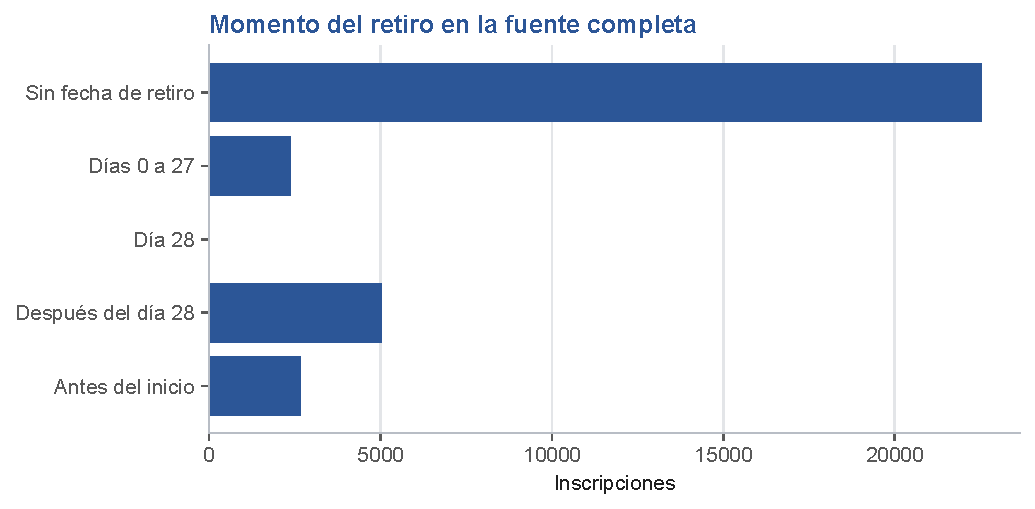
\includegraphics[width=.94\linewidth]{../figuras/01_momento_retiro.pdf}
\caption{Conteos de la fuente completa. El día 28 se mantiene separado de los eventos futuros.}\label{rev01:figretiro}\end{figure}
\section{Conclusiones y productos de la fase}
La estructura relacional permite integrar las fuentes sin pérdidas en las claves
auditadas. Sin embargo, la interpretación temporal exige distinguir retiros ya
ocurridos, resultados finales discordantes y disponibilidad de las evaluaciones.
El log contiene repeticiones cuya causa no es identificable en los archivos; conservar
el volumen original constituye una decisión de procesamiento documentada y su efecto
se acompaña de un escenario de sensibilidad.

La fase entrega una base de auditoría, un panel diario de clics y entregas con
metadatos. Las tablas completas, las huellas de archivos y las comprobaciones de
integridad se exportan junto con el notebook. Estos productos sustentan la preparación
de variables; no acreditan todavía la validez de un clasificador ni el desempeño de
un sistema de alerta temprana.

\section{Distribución temporal del retiro}
La figura presenta las 10\,072 inscripciones con fecha de retiro de toda la fuente. Los 2\,678 retiros preinicio no son eventos futuros de las ventanas examinadas; este denominador no debe mezclarse con la población filtrada por matrícula.

\begin{figure}[htbp]\centering
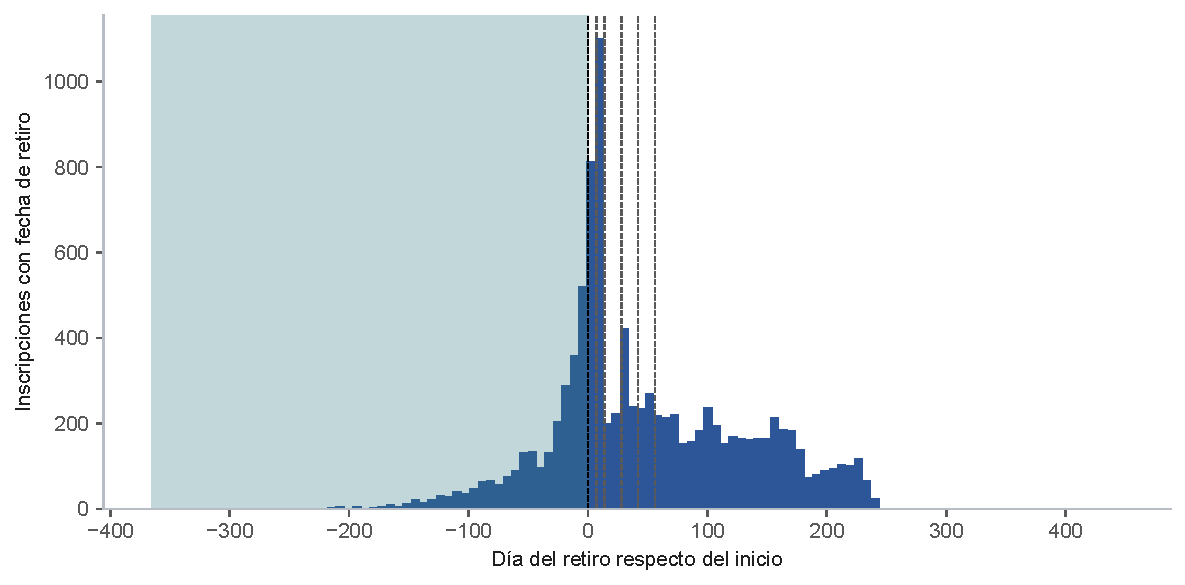
\includegraphics[width=.94\linewidth]{../figuras/01_fechas_retiro.pdf}
\caption{Distribución de fechas de retiro; líneas en el inicio y en los cortes 7, 14, 28, 42 y 56.}\label{corr:histograma}\end{figure}
